\section{Experiments}
We setup two environments in the grid world and windy grid world.
\subsection{Four room grid world}

Four room grid world is a grid world with four rooms connected to each other as shown in Figure~\ref{fig:four-room-grid-world}.

\subsection{Four room windy world}

Four room windy world is a grid world with four rooms connected to each other as shown in Figure~\ref{fig:four-room-grid-world}.
Some of the grid cells in have wind shown by arrow and the agent gets pushed around by
the wind with 0.25 probability irrespective of the action taken.

\subsection{Metrics}
We describe our metrics.

\subsubsection{Latency-1:1}

\subsubsection{Distance Inefficiency}


%
\begin{figure}%
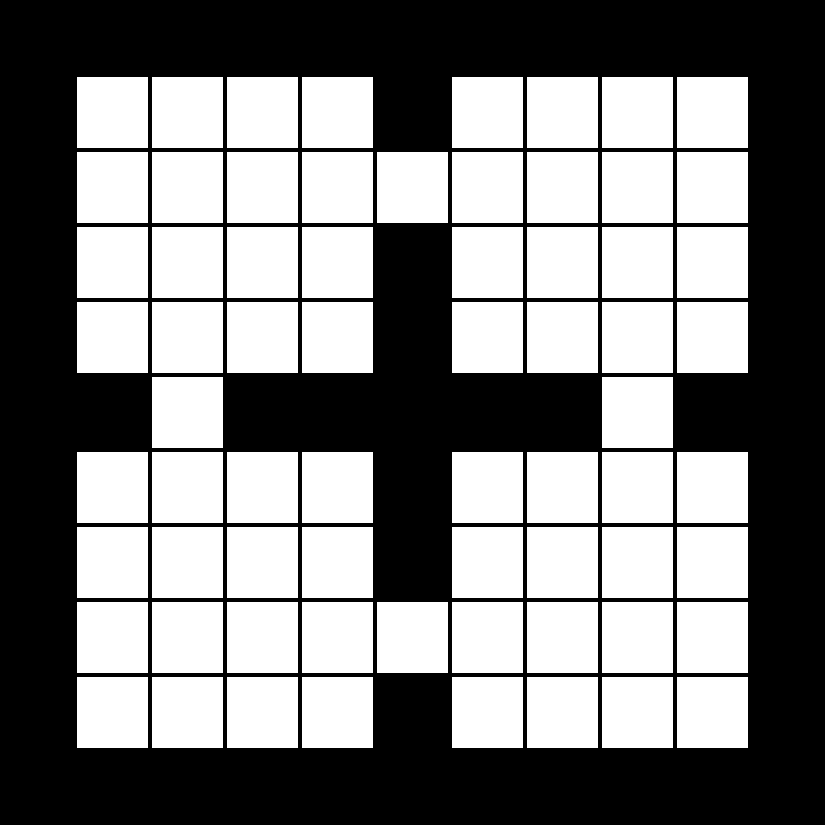
\includegraphics[width=0.48\columnwidth]{media/4-room-grid-world.pdf}
\hfill
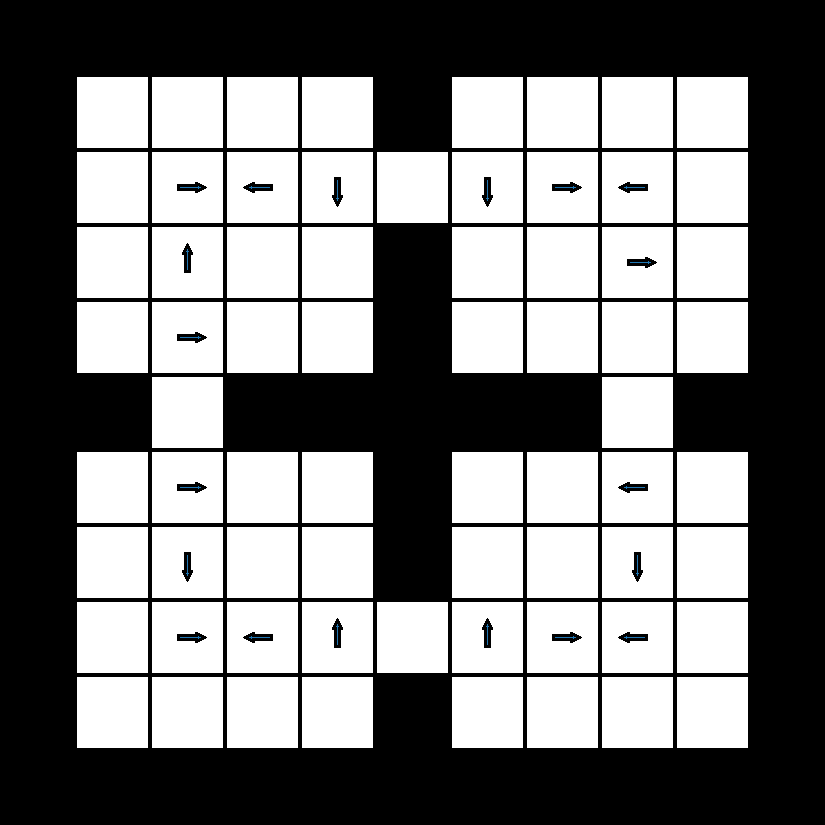
\includegraphics[width=0.48\columnwidth]{media/4-room-windy-world.pdf}%
\caption{Left: Four room grid world. Right: Four room windy grid world with wind direction shown by arrows. The windy pushes the agent in the direction of wind with 0.25 probability irrespective of the action taken.}
\label{fig:four-room-grid-world}%
\end{figure}%

